\documentclass[12pt]{article}
\usepackage[utf8]{inputenc}
\usepackage[T1]{fontenc}
\usepackage{amsmath}
\usepackage{amsfonts}
\usepackage{amssymb}
\usepackage[version=4]{mhchem}
\usepackage{stmaryrd}
\usepackage{hyperref}
\usepackage{graphicx}
\hypersetup{colorlinks=true, linkcolor=blue, filecolor=magenta, urlcolor=cyan,}
\urlstyle{same}

\begin{document}
These are problems meant to expand upon lecture. 

\section{}
Using the internet for help, sketch the real and imaginary parts of the dielectric function over a $10^0$ to $10^{15} \mathrm{~Hz}$ range for:
\subsection{}
An atom
\subsubsection{Answer}
For a single atom, the only thing we need to consider are electronic excitations.
\subsection{}
A multiple atom molecule
\subsubsection{Answer}
For a multiple atom molecule, we need to consider electronic, vibrational, and rotational excitations.
\subsection{}
A solid
\subsubsection{Answer}
For a solid, we need to consider phonons (vibrational) and electronic excitations.
Acoustic phonons are purely vibrations and optical phonons are when you have a photon coupled to a phonon. The optical phonons are the ones that will have a higher frequency, i.e., higher energy.\\
\begin{figure}[h]
\centering
\includegraphics[width=\textwidth]{dielectrics_v2.jpg}
\caption{Dielectric function for an atom, a multiple atom molecule, and a solid.}
\end{figure}
Features do not need to be exact or to scale. Label the key excitations that are present in each system. Hint: What rotational, vibrational, and electronic excitations are possible for each?

\section{}
A superposition state exists between the electron-hole excitation and the laser exciting field on a few femtosecond timescales, which we call coherence. Dephasing is the term we use to describe how scattering processes decohere the electron-hole pair wavefunction to be out of phase with the driving frequency. For the following systems, label what dephasing mechanism is present with the knowledge that electron-electron scattering is faster than electron-phonon scattering, which is faster than electron-spin/nucleus coupling. Like Problem 1, consider the possible excitations for the system.
\subsection{}
An atom
\subsubsection{Answer}
There are no free electrons here to scatter, so the longest coherence time. We can just have the electron-spin/nucleus coupling here, whic is the slowest scattering mechanism.
\subsection{}
A diatomic species
\subsubsection{Answer}
We have introduced the potential for vibrations so with respect to the single atom, so this will have a slightly shorter coherence time. It should be noted that this cannot be called phonons, as that term is reserved for vibrations in a lattice.
\subsection{}
A multiple atom molecule
\subsubsection{Answer}
There are more potential vibrations here with respect to the diatomic, so this will have a slightly shorter coherence time. We can also consider rotations here, but since the frequency ordering of electronic, vibrational, and rotational, go, respectively, as UV, IR, and then microwave in decreasing frequency, the rotations are the slowest and least energetic scattering mechanism.
\subsection{}
A semiconductor
\subsubsection{Answer}
We have introduced the potential for free carrier electrons here if we have excited across the band gap, so this will have a slightly shorter coherence time than the multiple atom molecule. Phonons are also a possibility and we can be having these phonons scatter the electrons.
\subsection{}
A metal
\subsubsection{Answer}
There is no band gap to consider here, so there will be much more scattering between electrons than for the semiconductor. As in the previous case, phonons are also possible.\\
So, the order is: Atom, Diatomic, Multiple Atom Molecule, Semiconductor, Metal.
I have also attached a figure \ref{fig:scattering} that gives some possible scattering mechanisms and their life times after an initial laser pulse:
\begin{figure}[h]
\centering
\includegraphics[width=\textwidth]{scattering.png}
\caption{Scattering mechanisms and their life times after an initial laser pulse.}
\label{fig:scattering}
\end{figure}
\newpage

\section{}

We do not have time to talk about semiconductor junctions in class.
\subsection{}
Research and draw an n-type Metal-Semiconductor Schottky barrier, a p-n junction, and a p-type Metal-Oxide-Semiconductor junction. 
\subsubsection{n-type Metal-Semiconductor Schottky barrier}
The mismatch in the metal and semiconductor Fermi levels before the formation of the junction is shown in the diagram labeled as before. The first thing that happens when they come into contact is electron density moves from the semiconductor to the metal (labeled 1). So once a photoexcitation occurs, leaving a hole in the semiconductor valence band and an electron in the conduction band, this hole wants to move towards the electron density that was previously built up in the metal (labeled 2). This process is shown in Figure \ref{fig:schottky}.
\begin{figure}[h]
\centering
\includegraphics[width=\textwidth]{schottky.jpg}
\caption{n-type Metal-Semiconductor Schottky barrier.}
\label{fig:schottky}
\end{figure}
\subsubsection{p-n junction}
For the second junction, just consider the p-type semiconductor undergoing a photoexcitation. Ordinarily, if we just created an electron-hole pair in the p-type semiconductor, it would be short-lived, i.e., we would be dealing with recombination effects. However, the n-type semiconductor provides us with an efficient avenue to prevent these recombination effects because the electron is moving away from the hole as it relaxes along the conduction band into the n-type semiconductor. The intermediate region in which the bands are bending is called the depletion layer, and we will have a net positive charge on the side of the p-type semiconductor and a net negative charge on the side of the n-type semiconductor. This process is shown in Figure \ref{fig:pn}.
\begin{figure}[h]
\centering
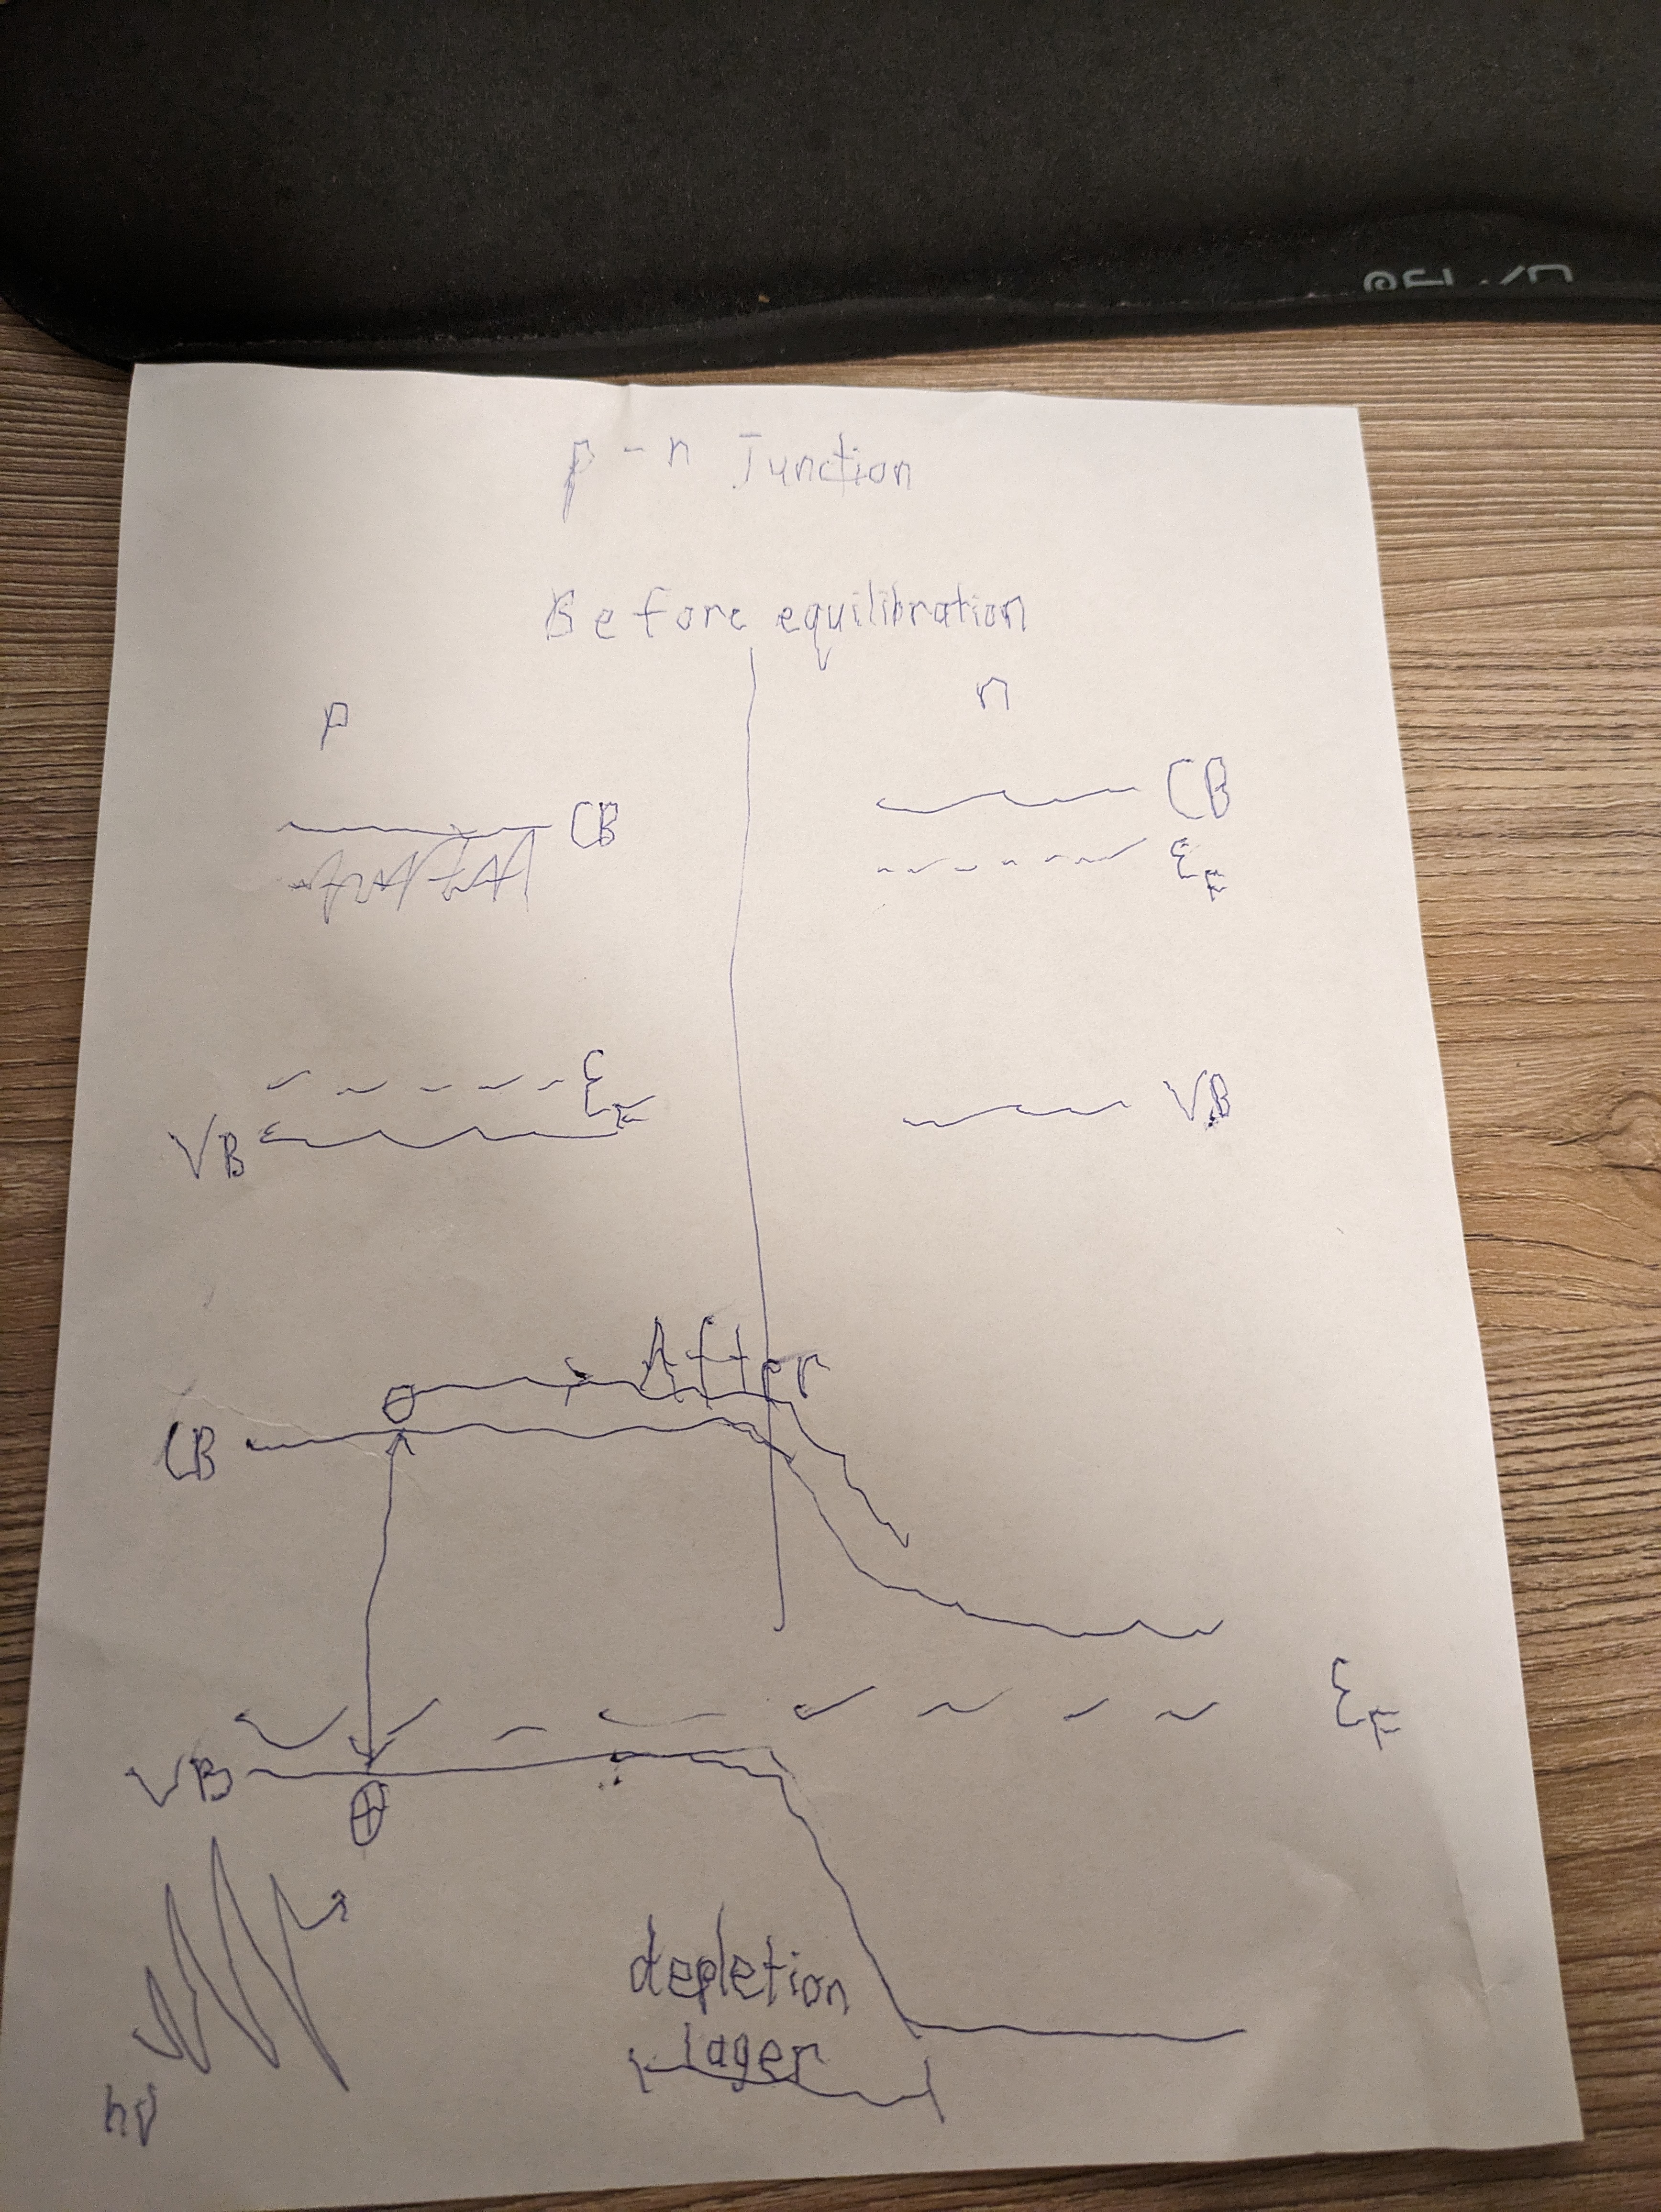
\includegraphics[width=\textwidth]{pn.jpg}
\caption{p-n junction. Do I get extra credit for drawing such a good photon lol}
\label{fig:pn}
\end{figure}
\subsubsection{p-type Metal-Oxide-Semiconductor junction}
We start by equilibrating the metals Fermi level with that of the semiconductor, which brings about an initial transfer of electron density from the metal, which has its Fermi level moving downwards, towards that of the semiconductor (labeled 1). When a photoexcitation occurs (labeled 2), that excited electron wants to move to a lower energy towards the metal, but the oxide barrier prevents it from doing so and in order to surmount this barrier a voltage difference needs to be introduced. This process is shown in figure \ref{fig:mos}.
\begin{figure}[h]
\centering
\includegraphics[width=\textwidth]{mos.jpg}
\caption{p-type Metal-Oxide-Semiconductor junction.}
\label{fig:mos}
\end{figure}
\subsection{}
For each junction, draw how photoexcited electrons and holes will move assuming only the semiconductor is photoexcited. Again, use the internet for help.\\



Extended Resource for Problem 3: If you want to calculate this for real in a paper, the freely available AFORS-HET software will calculate band bendings, alignments, photoexcited changes, etc., if you give it basic parameters like the work function, band gap, and dopants.

\href{https://www.helmholtz-berlin.de/forschung/oe/ee/si-pv/projekte/asicsi/afors-het/index}{https://www.helmholtz-berlin.de/forschung/oe/ee/si-pv/projekte/asicsi/afors-hhet/index}


\end{document}